% !TEX root = DesignDocument.tex

\chapter{Design  and Implementation}

\section{Systems Goals}
The goal of this system is to establish a tool chain between CAD files and AR hardware. To this effect, the system must provide a web interface for users to upload CAD files to the cloud to be converted to file types render-able by AR hardware for on-demand downloading and rendering by AR devices.  

\section{System Overview and Description}
%Provide a more detailed description of the major system components without getting too detailed.  This section should contain a high-level block and/or flow diagram of the system highlighting the major components. See Figure~\ref{systemdiagram}. This is a floating figure environment. \LaTeX\ will try to put it close to where it was typeset but will not allow the figure to be split if moving it can not happen.  Figures, tables, algorithms and many other floating environments are automatically numbered and placed in the appropriate type of table of contents.  You can move these and the numbers will update correctly.
CAD software and AR hardware are assumed available for use of this platform. CAD file support for AR headsets is also a standard for current manufacturers. Thus, the three primary components of this platform are a web interface, file conversion software, and mobile app. The website is intended to drive both the upstream and downstream of data flow. The upstream will be from the user to the cloud. The downstream will be from the cloud to AR devices via QR code or direct download. Between these data streams rests file conversion software that will be used to convert input files to output file types necessary for specific AR hardware. The website must also include a QR code generator plugin that will be used for generating unique QR codes to associate with uploaded files. Custom AR file viewing is not conveniently supported with common features for mobile devices and a companion app for this platform must be developed. See \ref{fig:UMLSystemOverview} for a visual representation of the interacting components of this platform.

\begin{figure}[H]
	\centering
	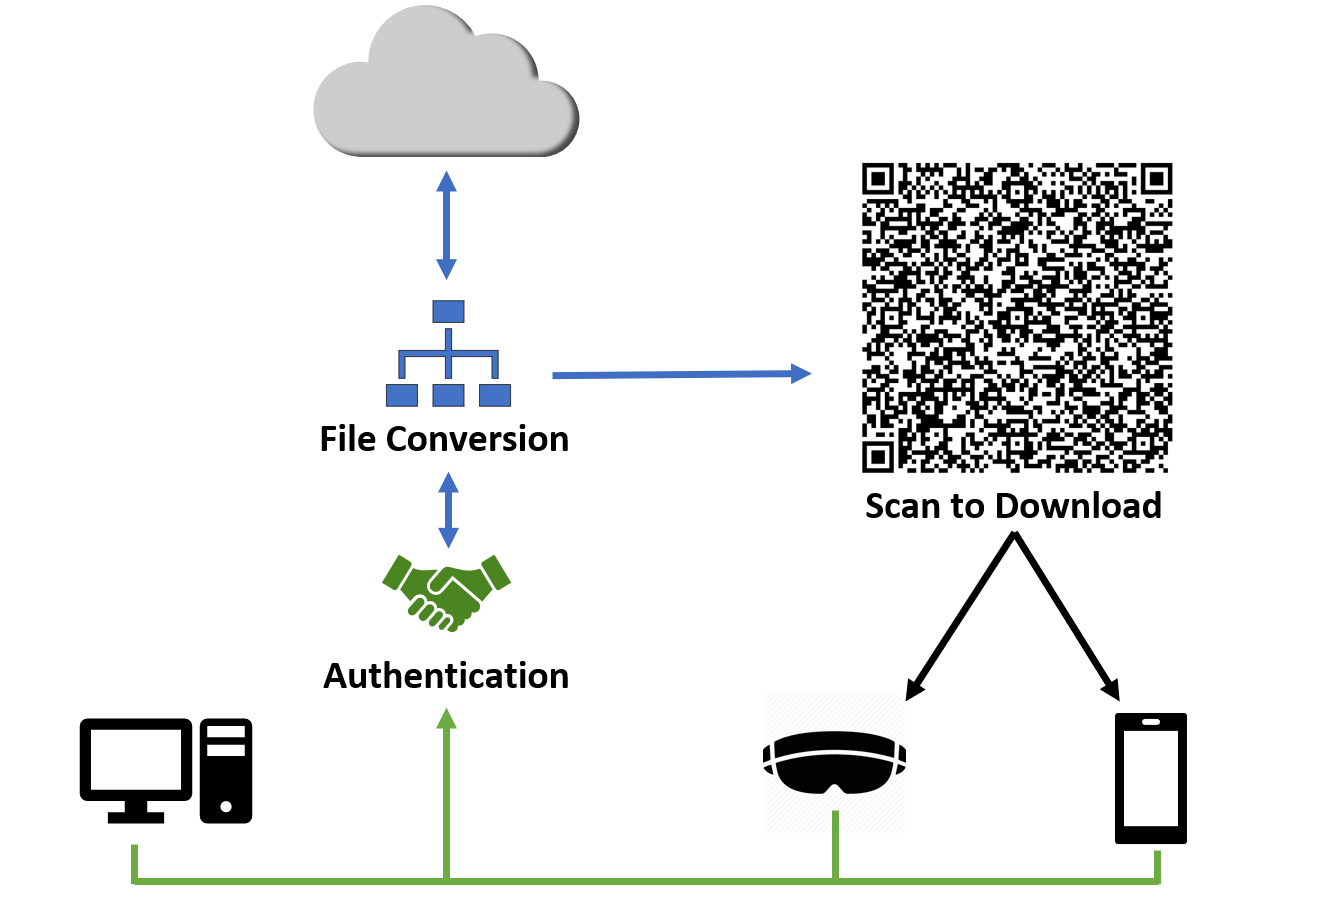
\includegraphics[width=\textwidth]{DataFlowDiagram.png}
	\caption{System Overview Diagram} 
	\label{fig:UMLSystemOverview}	
\end{figure}

\subsection{Website}
%Describe briefly the role this major component plays in this system. 
This major component of the system will broker all interactions occurring across the platform. A user interface will be used to control the data upstream between the user and the cloud. Functionality will include uploading, updating, and deleting files. The website will provide QR code generation for uploaded files and create an association between an uploaded file and its QR code. Note, a target file type must be specified when generating a QR code. When a direct download link or QR code download link is used, the cloud will supply a file in its specified format to the calling device. 


\subsection{File Conversion}
The file conversion software converts files between common 3D file types. It is designed to be called from the back end of the website.

Table \ref{tab:suportedfiletypes} lists the minimum file types supported.  More may be supported, but those listed are the minimum needed to support the majority of common file types.  
Models created in most common Computer Aided Design software can export to some of the input file types.

\begin{table}[!h]
    \centering
    \begin{tabular}{| c | c |}
        \hline
        Input file type & Output file type \\
        \hline
        .fbx & .fbx \\
        .dae & .dae \\
        .blend & .obj \\ 
        .obj & .stl \\
        .stl & .ply \\
        .ply & \\
        \hline
    \end{tabular}
    \caption{Supported File Types}
    \label{tab:suportedfiletypes}
\end{table}

\subsection{Mobile Device}
Mobile devices such as phones and tablets are able to download and view 3D files from the website. In the Android app, users can log in and see a listing of their private files, as well as scan QR codes to access additional files. Selecting one of these files allows them to view it in AR on the device. The Android app uses OBJ files retrieved from the website.

\subsection{HoloLens}
The HoloLens is a standalone AR device with advanced features and built-in software. The QR code reader software on the HoloLens can be used to scan a QR code and get a link to the file from the website. After downloading this file, the HoloLens user can view and interact with the model in an AR environment with the default viewer from Microsoft. The HoloLens uses FBX files retrieved from the website.

 \section{Architecture and System Design}
%This is where you will place the overall system design and the architecture.   This section will be very detailed and should be image rich.  There is the old phrase {\it a picture is worth a thousand words}, in this class it could be worth hundreds of points (well if you sum up over the entire team).   One needs to enter the design and why a particular design has been done.   THIS IS THE CORE OF THE COURSE.    
 
 
% {\it It is important for you to say why as much as what.   }
 
   \subsection{Design Selection}
   \paragraph{}
 Many design tools and coding stacks were considered at the beginning of this project.
 The main decisions we had to make were was our development environment and the cloud services.
 
 \paragraph{}
 The first thing that was decided on was the hosting tools.
 We decided on using the Azure cloud hosting tools for the following reasons.

 \begin{itemize}
    \item Allows for simple database and web hosting.
    \item Paid features are offered free to students.
 \end{itemize}

 We also debated on the coding stack to use for the website.
 We went with ASP.NET MVC for the following reasons:
\begin{itemize}
    \item A majority of the developers were familiar with C\# and Visual Studio.
    \item The decision to use Azure made ASP.NET MVC a natural choice, since they are both part of the Microsoft stack.
\end{itemize}

\paragraph{}
The other options we explored were Amazon Web Service for cloud hosting and linux development environment using Python and Django for the back-end logic.
We didn't pursue these because negative feedback from our own developers as other professional reviews.

 \subsection{Data Flow}
The web interface for users creates a data upstream exists between a web browser and a cloud server. Users may upload, update, and delete remotely hosted files.

Data downstream exists between the cloud server and AR hardware. Data downstream is initiated by users calling file download through QR codes or direct download links. 

When a file us upload, a QR code generator plugin will be activated to generate and deliver a unique QR code to the web interface to be downloaded by the user and stored on the cloud server in association with the related file. 

When a file is accessed by an AR device, conversion software will convert the file to the appropriate AR compatible file type before delivery. This converted file will be stored on the cloud server for a limited time to streamline repeated and multi-user access.
  
\subsection{UML}
 
	\begin{figure}[H]
	 	\centering
		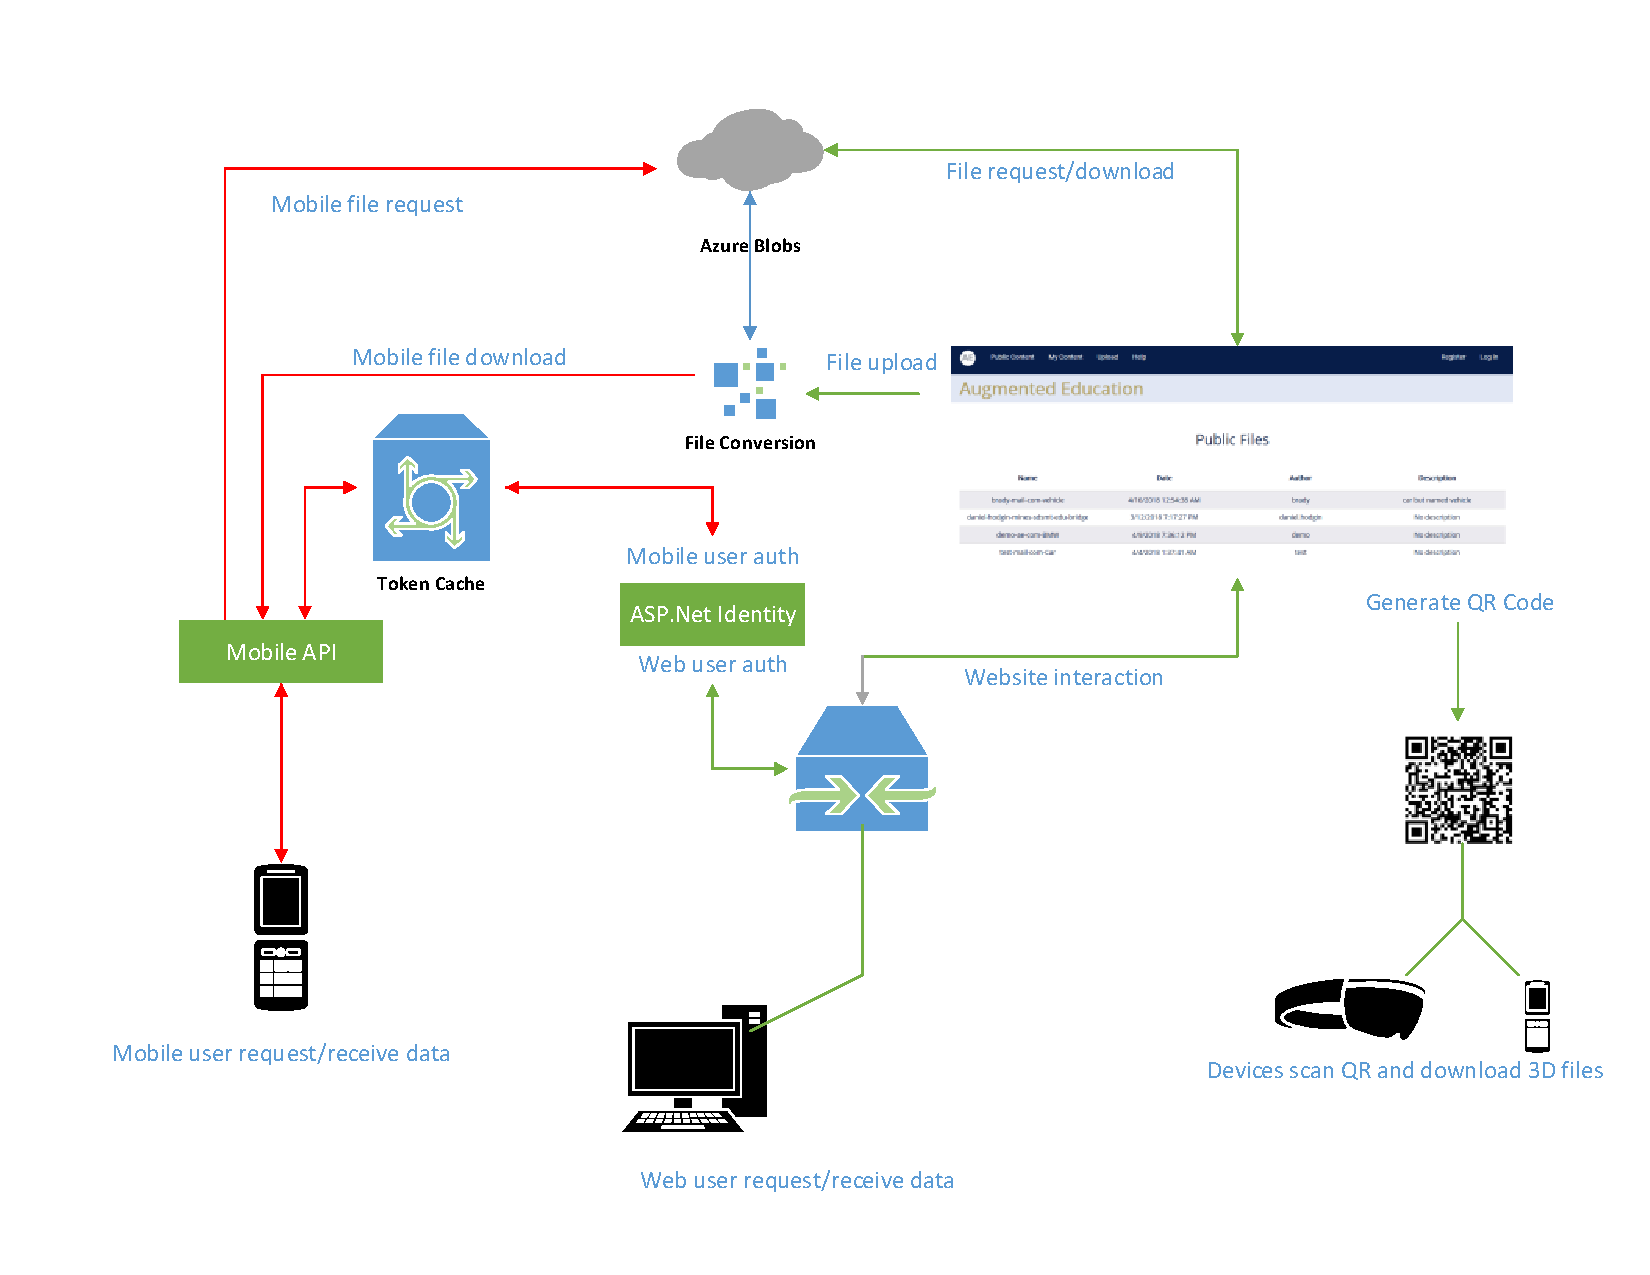
\includegraphics[width=\textwidth]{UML.pdf}
		\caption{System UML Diagram} 
	 	\label{fig:SystemUML}	
	\end{figure}
    
\subsection{UX}

Upon delivery of the MVP, user experience testing will be conducted once per sprint with five representative client faculty members: Dr. Jeff McGough, Dr. Christer Karlsson, Dr, Adam Piper, Dr. Brent Deschamp, and Dr. King Adkins. User experience testing will include inspection of the elements including, but not limited to, the following:

\begin{itemize}
	\item Appearance
	\item Ease of use
	\item Help and guidance features
	\item Ease of locating control features and elements of interest
	\item Speed of content delivery 
\end{itemize}



 \section{Website}

 \subsection{Overview}
 \paragraph{}
 The website is a hosting service for uploading, downloading and managing the users files. Microsoft's ASP.NET MVC was used to create the website and Azure was used for its web hosting and file storage tools.
 
 \paragraph{}
 Users can create an account to store and share 3D models with other users. Once a user has an account, they can upload a 3D model as one of the websites supported file types. A user can download the model as any of the supported file types or generate a QR code that can be used for quick download using the mobile app or any other QR code readers.

\subsection{User Interface}
The user interface was designed to be very simple. The UI is comprised of four main pages with a navigation bar to get the pages
    \paragraph{Public Content Page}

        \begin{figure}[H]
        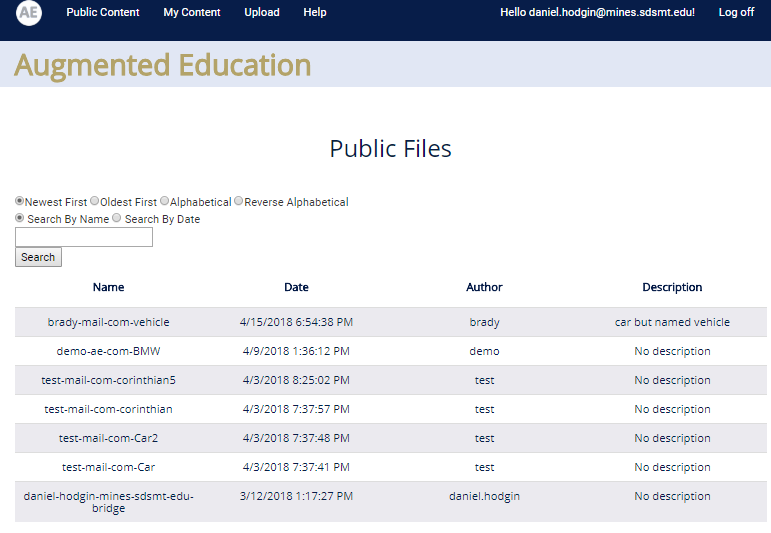
\includegraphics[width=0.5\textwidth]{Web/PublicPage}
        \centering
        \caption{Public Content Page}
        \label{fig:PublicContent}
        \end{figure}

        This is the main landing page for the website. From here users are able to browse the public files to download and generate QR code. Users do not need to be signed in or have an account to access the information on this page.

    \paragraph{My Content Page}
        \begin{figure}[H]
        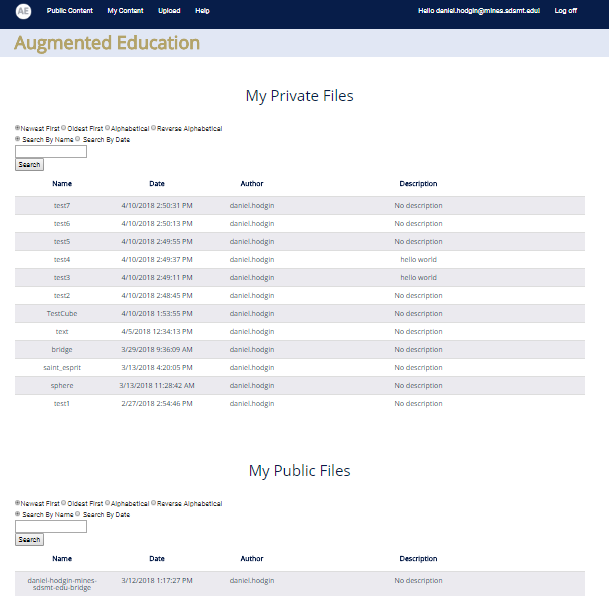
\includegraphics[width=0.5\textwidth]{Web/MyContent}
        \centering
        \caption{My Content Page}
        \label{fig:MyContent}
        \end{figure}

        This page will display all of the content that a user has uploaded. Here a user can browse their private and public files to download and generate QR codes. Users also have the ability to delete files. Users must have an account to access this page.

    \paragraph{Upload Page}
        \begin{figure}[H]
        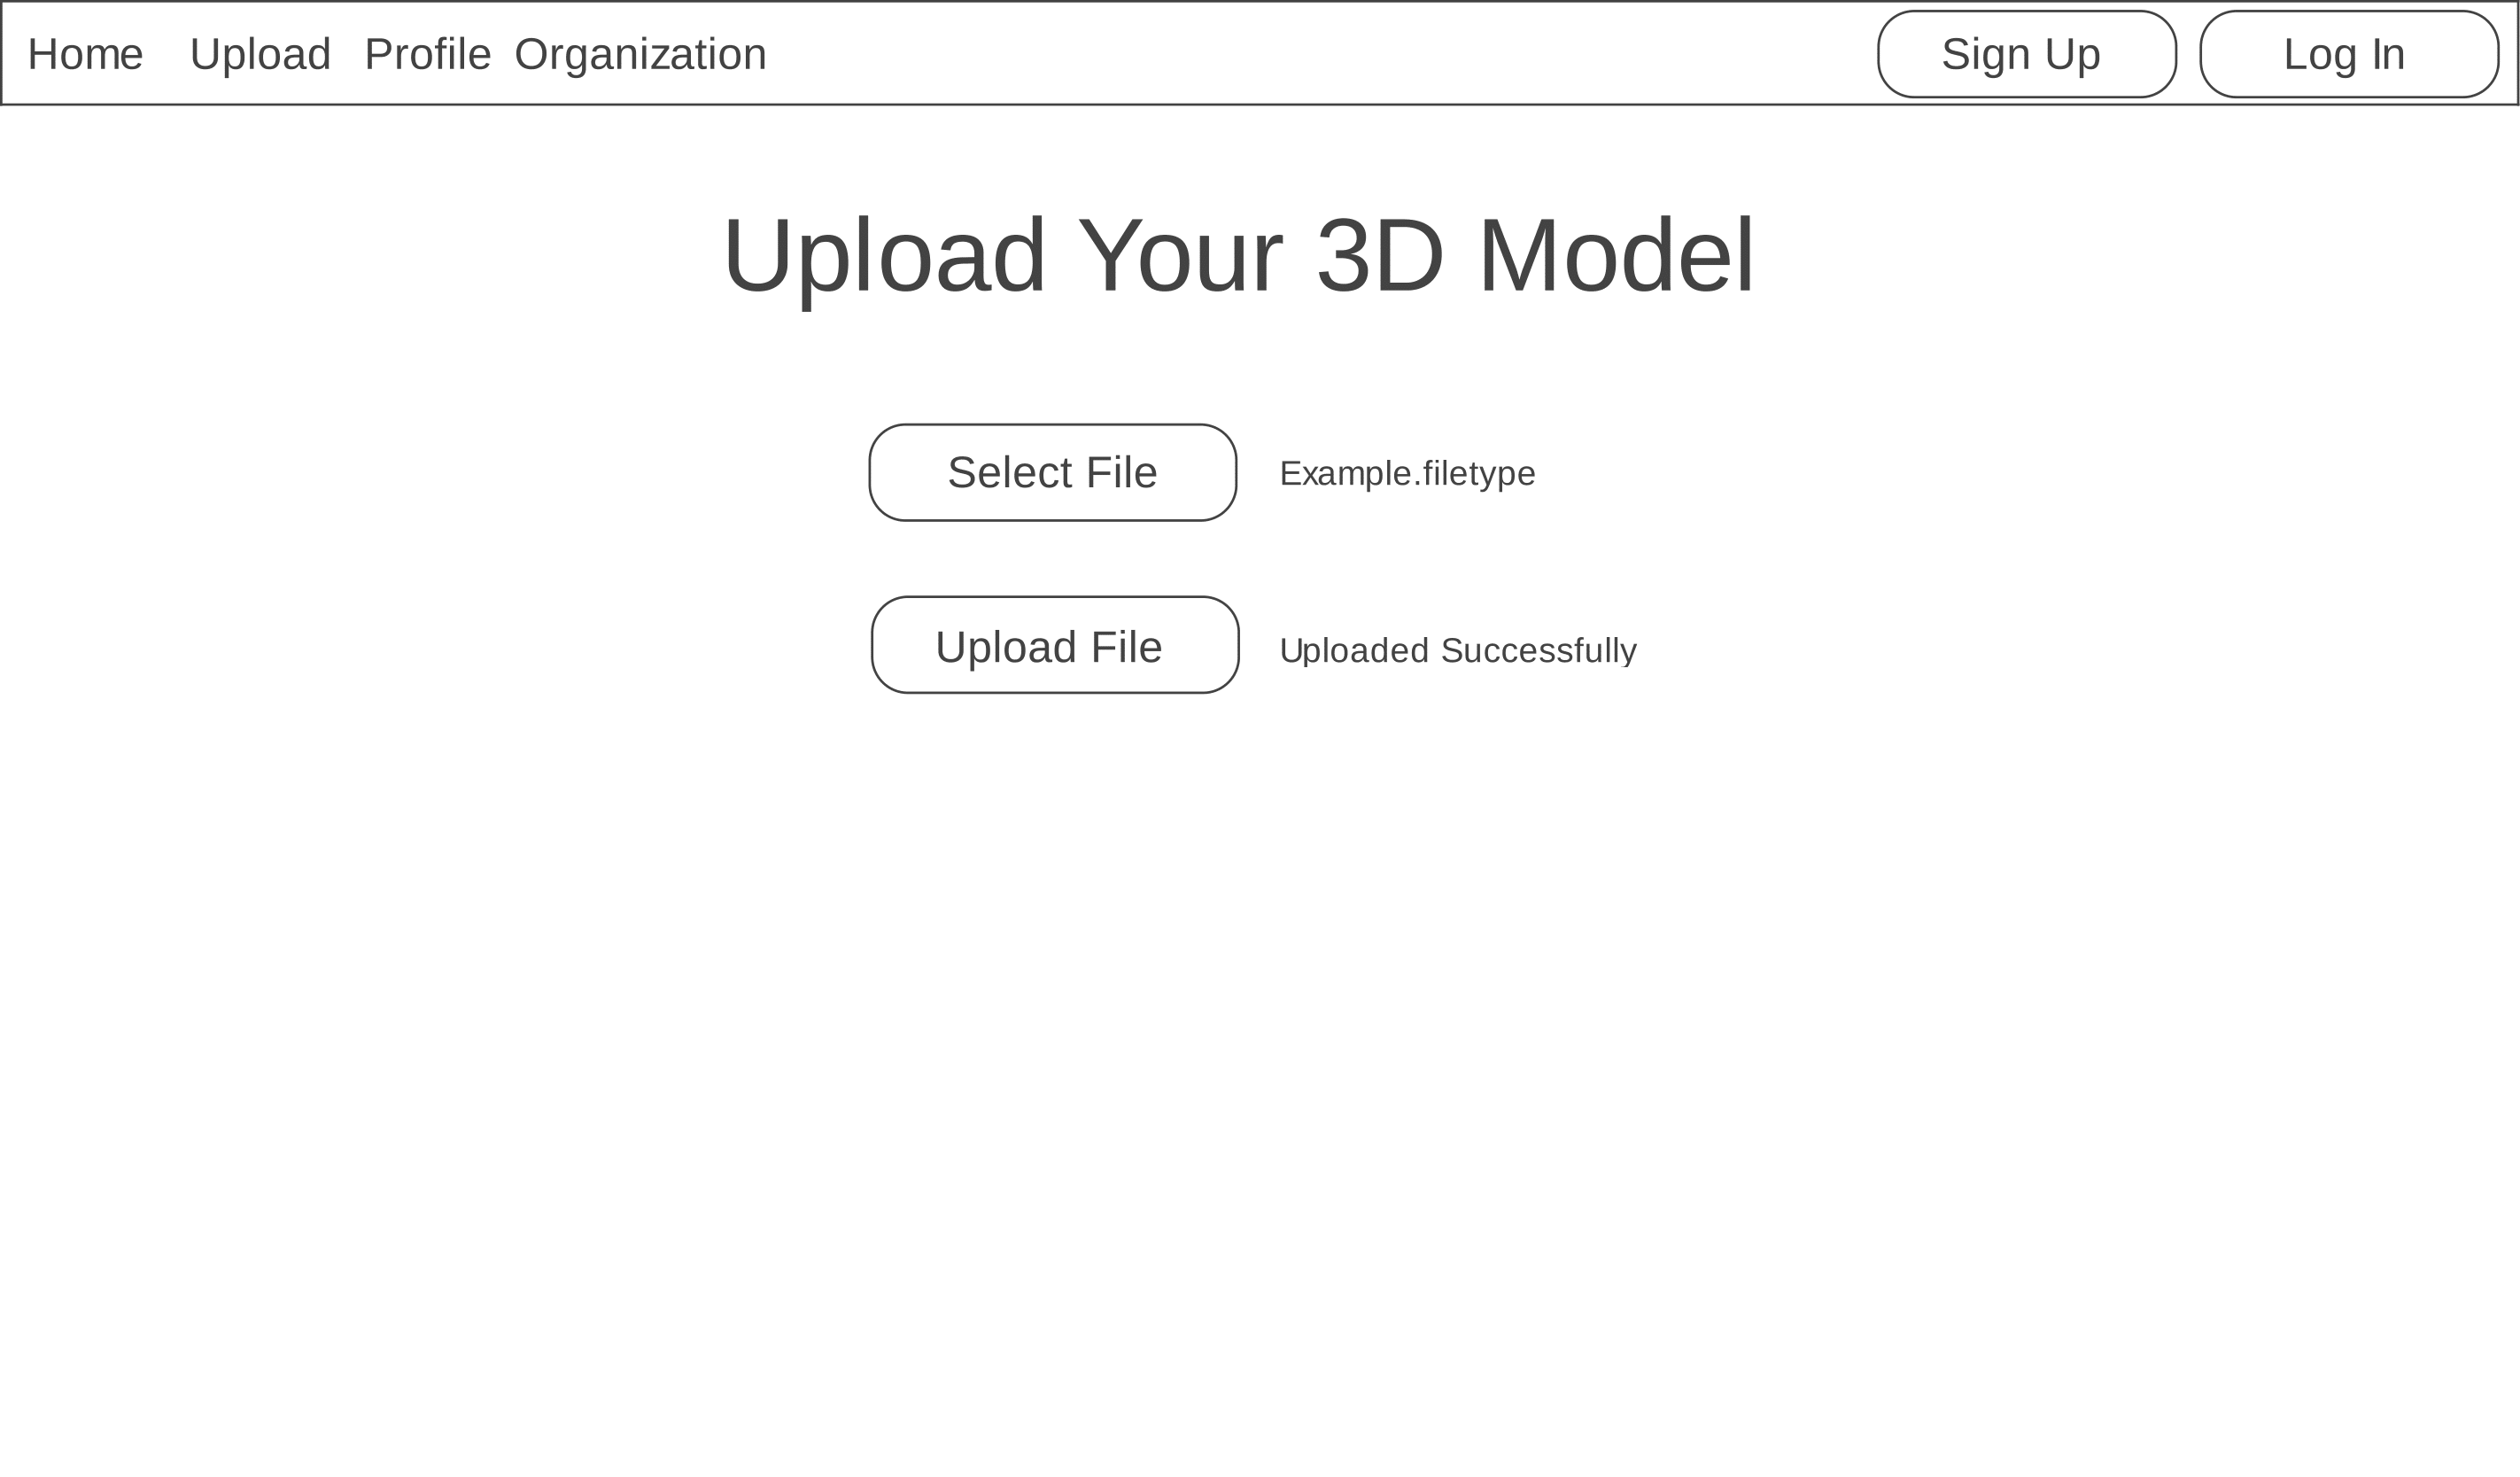
\includegraphics[width=0.5\textwidth]{Web/Upload}
        \centering
        \caption{Upload Page}
        \label{fig:UploadPage}
        \end{figure}

        This page will allow users to upload 3D models. Users can upload a material file if it is an OBJ file. The user can add a description, specify an alternate name, and make the file public. Users must have an account and be signed in to access this page.

    \paragraph{Help Page}
        \begin{figure}[H]
        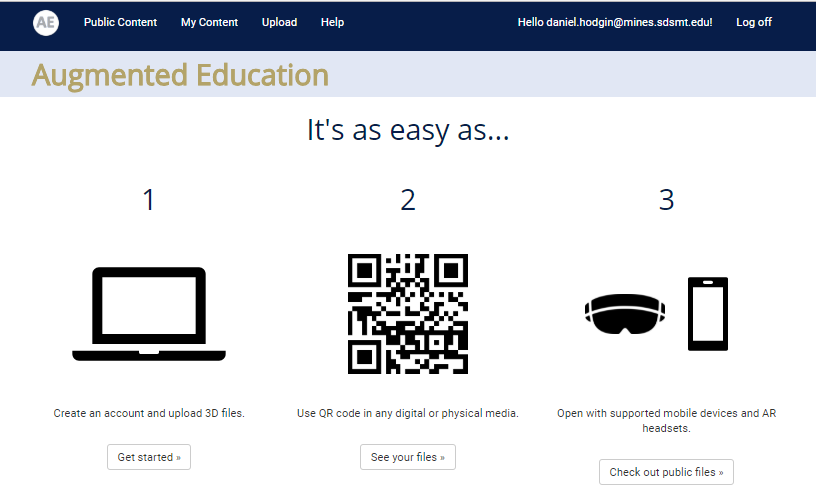
\includegraphics[width=0.5\textwidth]{Web/Help}
        \centering
        \caption{Upload Page}
        \label{fig:HelpPage}
        \end{figure}
    
        This page just gives a simple tutorial on how to uses the website.

\subsection{Technologies Used}

    As stated earlier in this document, this product is making use
    of the Microsoft environment for its tools. Below is an in-depth 
    breakdown of the tools currently being used:

    \begin{itemize}
    \item ASP.NET MVC
    \begin{itemize}
        \item An MVC web architecture, where the backend logic is written in controller classes
        that send and receive data from the client.
        \item It allows for dynamic html pages using a Razor syntax. Razor allows
        you to embed C\# Code into the html and execute logic.
    \end{itemize}
    
    \item Azure
        \begin{itemize}
            \item Microsoft cloud hosting services.
            \item Allows for simple database and web hosting.
            \item Paid features are offered free to students.
        \end{itemize}
    \end{itemize}

    These tools make up the core development of this website. The website is also
    making use of other smaller packages to handles user authentication and database management.

    The website also implements the file conversion software that is described later.
    The file conversion was written in C++, so it couldn't be compiled with the website.
    The workaround was that the file conversion was compiled into an executable that can be used through a system command to convert the file.


    \subsection{Data Flow}
    The website acts as an intermediary between the user and the cloud. Data flow for the website can be broken into a upload and download data flow.

    \paragraph{Upload Data Flow}
    \begin{itemize}
        \item Once a user upload a file it is temporarily save on the server.
        \item If the file is not a FBX file it is converted to a FBX file.
        \item The file is then uploaded to Azure blob storage for long term storage.
        \item The file on the server is then deleted on a sucessful upload to Azure.
    \end{itemize}

    \paragraph{Download Data Flow}
    \begin{itemize}
        \item When a user requests to download a file or generate a QR code, the file name and type is sent to the server.
        \item The server pulls the file from Azure and temporarily save it to the server.
        \item If a download is requested, it does a conversion if nessessary and send the file to the user.
        \item If a QR code is generated, it does a conversion if nessessary and then saves it back to Azure storage and returns a link to the file in Azure embedded in a QR code.
        \item 
    \end{itemize}


\subsection{Design Details}

    \subsubsection{Overview}

    The website was written in C\# with the ASP.NET MVC framework. The main logic
    of the website are contained in two controllers
    \begin{itemize}
        \item Upload Controller
        \begin{itemize}
            \item Handles upload from client to the server.
            \item Uses File Conversion executable to convert to .fbx
            \item Stores file on the web.
        \end{itemize}
        \item Download
        \begin{itemize}
            \item Uploads Model tag from client to server.
            \item Finds associated store model.
            \item Returns model to the client.
        \end{itemize}
    \end{itemize}

    \subsubsection{Code Structure}
    As stated before the website is using ASP.NET MVC framework. 
    The logic happens in the controllers and is split up into the upload and download controller.
    
    \paragraph{Parameter Passing}
    \hfill \break
    The main functions that are being used are the upload and download function.
    
    \begin{itemize}
        \item Upload Function
        \begin{itemize}
           \item HttpPostedFileBase - http message sent from client to server containing the file
           \item The message is parsed to retrieve the file and save to the web.
        \end{itemize}

        \item Download Function
        \begin{itemize}
            \item input string ModelTag - string containing the reference tag to the model.
            \item output httpresponse - http message sent from server to client containing the file. 
        \end{itemize}
    \end{itemize}

 \section{File Conversion}

    \subsection{Overview}
    \paragraph{}
    A major tool in the project is the file conversion software.  
    The file conversion software aims to read in many different 3D model file types (.fbx, .obj, .dae, etc.) and convert them to another desired 3D file types.  
    A brief listing of supported file types is in table \ref{tab:suportedfiletypes}.
    
    \paragraph{}
    This tool is intended to be used on the back end of the website.  Whenever a user uploads a file, it can be converted to a common file type.
    When the user requests a download on an AR device, the type may be different than what is stored. Therefore, the tool will be used to convert the file before
    it is sent to the user.
    
    \paragraph{}
    Since this tool is intended to be used on the backend of a website, it is appropriate to use a command line interface.  
    The flags that can be passed to the program are listed below:
    
    \begin{table}[h]
        \centering
        \begin{tabular}{l  l}
            \texttt{-i} & Input file name (can specify full path), infers the input file type from the name \\
            \texttt{-o} & Name (or full path) to write the converted file, infers the export file type from the name \\
            \texttt{-odir} & The path to the directory, the file name is inferred from the input file name \\
            \texttt{-t} & The file type (.fbx, .obj, .dae, etc.) to export to
        \end{tabular}
    \end{table}
    
    Note the \texttt{-t} flag is only needed when using the \texttt{-odir} flag.  The \texttt{-odir} just specifies which directory to write to, but not the file type.
    Therefore, more information is needed in order to export to a file.  The \texttt{-o} flag will parse the file name and extract the file type from the \texttt{-i} file name.
    
    An example command to run:
    
    \begin{center}
        \texttt{.\textbackslash FileConversion.exe -i C:\textbackslash SomePath\textbackslash someFile.obj -t fbx -odir C:\textbackslash SomeOtherPath\textbackslash}
    \end{center}
    
    This will convert a file named \texttt{someFile.obj} located at \texttt{C:\textbackslash SomePath\textbackslash  to an FBX file named someFile.fbx} located at 
    \texttt{C:\textbackslash SomeOtherPath\textbackslash}
    
    \subsubsection{File Type Research}

    The goal for the file type research was to find the common 3D model file types, and what is commonly used with AR devices.

    \paragraph{OBJ}
    The OBJ filetype (Wavefront OBJ) stores a list of vertices, and constructs faces using the vertices.  OBJ supports textures, applied to each face, that are stored in a separate MTL file.  Each face in the OBJ file can reference a material in the MTL file to provide the texturing needed. The MTL file can also reference PNG or BMP files for textures. The Android app uses files in the OBJ format.

    \paragraph{STL}
    The STL file type (sterolithography) stores a list of vertices and forms triangles to form the surfaces of an object.  This file type does not support textures.  It is commonly used in 3D printing.

    \paragraph{DAE}
    The DAE file type (Collada) uses XML to store a 3D model.  It supports textures and animations embedded in the file.  Therefore, a model with textures and/or animations are stored in a single file.

    \paragraph{FBX}
    The FBX file type (Autodesk FilmBox) is a proprietary file format for Autodesk.  It is commonly used, and is supported, by many different AR devices such as the HoloLens.

    \paragraph{Conculsions}
    The above file types were found to be the most common.  The intermediate file type was agreed to be DAE.  It supported the most features while encapsulating all the data in a single file.

    \subsection{Technologies Used}
    
    The code for the file conversion toolset is written in C++.  There are two main external libraries used:
    \begin{itemize}
        \item Open Asset Import Library (assimp)
        \begin{itemize}
            \item \url{http://assimp.org/main_downloads.html}
        \end{itemize}

        \item FBX SDK
        \begin{itemize}
            \item \url{http://usa.autodesk.com/adsk/servlet/pc/item?siteID=123112&id=26416244}
        \end{itemize}
    \end{itemize}

    Multiple libraries were needed to support the file types that were necessary for common AR rendering.  In the Microsoft HoloLens, the default
    3D viewer supports FBX files very easily.  Therefore, it was decided that the conversion software needed to export to FBX.  The best tool to do 
    so is the FBX SDK, since FBX is a proprietary file format from Autodesk.  However, the FBX SDK has a very limited range of file types it will read and write.
    Therefore, the Open Asset Import Library is used to better support a wide array of file types.  So in using assimp and the FBX SDK together,
    the conversion software can support a wide range of both import and export file types.

    \subsection{Data Flow}
        There are four main paths data can flow.
        \begin{itemize}
            \item assimp
            \begin{itemize}
                \item import and export all with the assimp library
            \end{itemize}
            
            \item FBX SDK
            \begin{itemize}
                \item import and export all with the FBX SDK library
            \end{itemize}

            \item assimp $\rightarrow$ FBX SDK
            \begin{itemize}
                \item import with assimp, export to temporary file type
                \item import temporary file with FBX SDK, export to final file 
            \end{itemize}

            \item FBX SDK $\rightarrow$ assimp
            \begin{itemize}
                \item import with FBX SDK, export to temporary file type
                \item import temporary file with assimp, export to final file 
            \end{itemize}
        \end{itemize}
        
        This outlines that the program tries to use a single library to convert the file before using both libraries.  If a single library is unable to 
        read and write the needed formats, it tries to import with one, export to a temporary format, and export with the other.  An example of 
        using a single library is if a user wants to read a .obj and write to a .fbx.  The FBX SDK can handle reading and writing those particular file
        types, so it will be used to do the conversion.  An example of needing to use both libraries is if a user wants to convert a .ply to a .fbx.
        assimp can read .ply files, but cannot write to .fbx.  The FBX SDK can write to .fbx files but not read .ply.  Therefore, assimp is used to 
        read the .ply, write to a .dae (common file type).  The FBX SDK then reads the .dae and writes to a .fbx.

    \subsection{Design Details}

    \subsubsection{Overview}

    The file conversion software was written in C++.  The structure of the program is object oriented, where classes are defined where the functionality needed
    in the program is defined.  Instances of the classes will be created when needed.  
    The high level view of the program is:
    \begin{enumerate}
        \item Parse command line arguments
        \item Convert the file
        \item Print error messages if errors occurred
    \end{enumerate}

    The parsing the command line arguments section may fail if the user does not supply the correct arguments.  A flag is set after parsing to indicate
    whether the correct arguments were supplied.  If an error occurs during file conversion, the error will be denoted by an integer error code.  
    During file conversion, if a single library could not convert it on its own, an extra file will be created as an intermediate file.

    \subsubsection{Code Structure}
    The file conversion software is broken into two main sections: parameter parsing and file conversion.

    \paragraph{Parameter Parsing}
    \hfill \break
    The parameter parsing code is in a class called ParseParameters.  ParseParameters has a constructor that takes the number of command line arguments, 
    and the command line arguments.  It will parse the values needed out into member variables that are public.  It will ignore invalid arguments,
    and print a usage statement if the correct arguments are not supplied.  When printing the usage statement, cout is used to write to standard out.

    After processing the command line arguments, the member variables in the class will be set with the appropriate information.  The member variables are:

    \begin{tabular}{l l}
        \centering
        success & bool \\
        & True if the needed information is set, false otherwise \\

        inputFile & string \\
        & The name/path of the file to convert \\

        outputFile & string \\
        & The name/path of the file to export to \\

        fileExtention & string \\
        & The file extension of the output file
    \end{tabular}

    If the success variable is false, the other member variables possibly have bad data that should not be used.

    \paragraph{File Conversion}
    \hfill \break
    The file conversion portion of the program is the meat of the functionality.  It takes an input file, and tries to convert it to the file type requested.
    This section implements the two libraries.  Each library is implemented in a class inherited from an abstract AbstractConverter converter class.  The two 
    library implementation classes are called AssimpConverter and FBXConverter.  A class named FileConverter contains the logic on determining which 
    library/libraries to use when converting the file.

    \subparagraph{AbstractConverter}
    \hfill \break
    The AbstractConverter is an abstract class that acts like an interface for the child classes.  The abstract methods are:
    \begin{itemize}
        \item SupportsInputFileType
        \begin{itemize}
            \item Return true if the converter can read in a file with a given file type
        \end{itemize}

        \item SupportsOutputFileType
        \begin{itemize}
            \item Return true if the converter can write to a file with a given type
        \end{itemize}

        \item ConvertFile
        \begin{itemize}
            \item Performs the file conversion
        \end{itemize}
    \end{itemize}

    An emum is defined, called Result, that provides a more self documenting way to return information from functions.  Values less than zero are errors, while
    value greater than zero are successes.  The levels of the enum are:
    
    \begin{tabular}{l l}
        \centering
        Failed &\\
        IOError &\\
        SceneNotLoaded &\\
        NotInitialized &\\
        FileTypeNotSupported &\\
        Success &
    \end{tabular}

    \subparagraph{AssimpConverter}
    \hfill \break
    The AssimpConverter inherits from the AbstractConverter and uses the Open Asset Import Library for file conversion.  
    The file type supported methods are implements by adding the supported file types to a set, and checking whether the questionable type is in the set.
    The list of file types supported is taken from the Open Asset Import Library website's list of supported input file types.  
    The output file types list comes from the same location.
    When converting a file, optimizations may be performed on the file to remove unnecessary/duplicate information.  For example, when importing a file, 
    repeated vertices in the meshes will be condensed into one, to help reduce the size of the file.

    \subparagraph{FBXConverter}
    \hfill \break
    The FBXConverter inherits the AbstractConverter and uses the FBX SDK to import and export files.
    THe file type input and output lists are derived from the FBX SDK website.

    \subparagraph{FileConverter}
    \hfill \break
    The FileConverter looks at the input and output file types, and determines which library/libraries needed to convert the file.
    It tries see if a single library can do the conversion.  If not, then both libraries are used by exporting from one into a 
    temporary file (.dae) and converting that to the final file type. After comparing the read/write lists between the libraries,
    the DAE file type was common between the two, and included features that other file types did not.  Therefore, it was chosen
    to have DAE as the common intermediate file type.

 \begin{comment}
    \section{Major Component \#1 }

    {\bf If the following makes sense, use this outline, if not then modify the outline}


    This section is used to describe the design details for each of the major components 
    in the system.    Note that this chapter is critical for all tracks.  Research tracks would do experimental design here where other tracks would include the engineering design aspects.    This section is not brief and requires the necessary detail that 
    can be used by the reader to truly understand the architecture and implementation 
    details without having to dig into the code.    Sample algorithm:  Algorithm~\ref{alg1}.  This algorithm environment is automatically placed - meaning it floats.   You don't have to worry about placement or numbering.  

    \begin{algorithm} [tbh]                     % enter the algorithm environment
    \caption{Calculate $y = x^n$}          % give the algorithm a caption
    \label{alg1}                           % and a label for \ref{} commands later in the document
    \begin{algorithmic}                    % enter the algorithmic environment
        \REQUIRE $n \geq 0 \vee x \neq 0$
        \ENSURE $y = x^n$
        \STATE $y \Leftarrow 1$
        \IF{$n < 0$}
            \STATE $X \Leftarrow 1 / x$
            \STATE $N \Leftarrow -n$
        \ELSE
            \STATE $X \Leftarrow x$
            \STATE $N \Leftarrow n$
        \ENDIF
        \WHILE{$N \neq 0$}
            \IF{$N$ is even}
                \STATE $X \Leftarrow X \times X$
                \STATE $N \Leftarrow N / 2$
            \ELSE[$N$ is odd]
                \STATE $y \Leftarrow y \times X$
                \STATE $N \Leftarrow N - 1$
            \ENDIF
        \ENDWHILE
    \end{algorithmic}
    \end{algorithm}
    Citations look like~\cite{Choset:2005:PRM, arkin2009governing, lavalle2006}  and~\cite{wiki:asimo,lumelsky:1987, nolfi2000evolutionary}.  These are done automatically.  Just fill in the database {\tt designrefs.bib} using the same field structure as the other entries.  Then pdflatex the document, bibtex the document and pdflatex twice again.  The first pdflatex creates requests for bibliography entries.
    The bibtex extracts and formats the requested entries.  The next pdflatex puts them in order and assigns labels.  The final pdflatex replaces references in the text with the assigned labels.
    The bibliography is automatically constructed.  
    


    \subsection{Technologies  Used}
    This section provides a list of technologies used for this component.  The details 
    for the technologies have already been provided in the Overview section. 

    \subsection{Component  Overview}
    This section can take the form of a list of features. 

    \subsection{Phase Overview}
    This is an extension of the Phase Overview above, but specific to this component. 
    It is meant to be basically a brief list with space for marking the phase status. 

    \subsection{ Architecture  Diagram}
    It is important to build and maintain an architecture diagram.  However, it may 
    be that a component is best described visually with a data flow diagram. 


    \subsection{Data Flow Diagram}
    It is important to build and maintain a data flow diagram.  However, it may be 
    that a component is best described visually with an architecture diagram. 


    \subsection{Design Details}
    This is where the details are presented and may contain subsections.   Here is an example code listing:
    \begin{lstlisting}
    #include <stdio.h>
    #define N 10
    /* Block
    * comment */
    
    int main()
    {
        int i;
    
        // Line comment.
        puts("Hello world!");
    
        for (i = 0; i < N; i++)
        {
            puts("LaTeX is also great for programmers!");
        }
    
        return 0;
    }
    \end{lstlisting}
    This code listing is not floating or automatically numbered.  If you want auto-numbering, but it in the algorithm environment (not algorithmic however) shown above.

\end{comment}


\section{Mobile App}

    \subsection{Overview}
The mobile app is used to visualize 3D models, accessing files from the website and scanning QR codes. It is an Android application using ARCore, Google's newest Augmented Reality library.
    \subsection{Technologies Used}
The Android app is developed in Android Studio, primarily with the Java programming language. The following libraries were used in this project.
    \begin{itemize}
        \item ARCore - Support for AR on Android devices (off of the Google Play Store)
        \begin{itemize}
            \item Only works on specific devices (as of 4/26/2018)
            \item Use OpenGL to draw models, ARCore only performs tracking/world mapping
        \end{itemize}
        \item Obj Parser
        \begin{itemize}
            \item Used by the example AR Core application to draw the model
            \item Parses the obj files
            % \item \url{https://github.com/JohnLXiang/arcore-sandbox}
        \end{itemize}
        \item QR Code Reader - included in Android project dependencies
        \item Volley - Google library for network communications between app and website
        \item Room - Google library that provides an abstraction layer over SQLite for storing file listings in the phone's database.
    \end{itemize}

    \subsection{Design Details}
    
    \subsubsection{Overview}
        
        The mobile app software is written in Android Studio in the Java programming language. It is an object oriented program with "activities" being the different screens that users can move between. The app has four main screens which are the login, file listing, QR code reader, and AR viewer.
        
        \begin{figure}[H]
            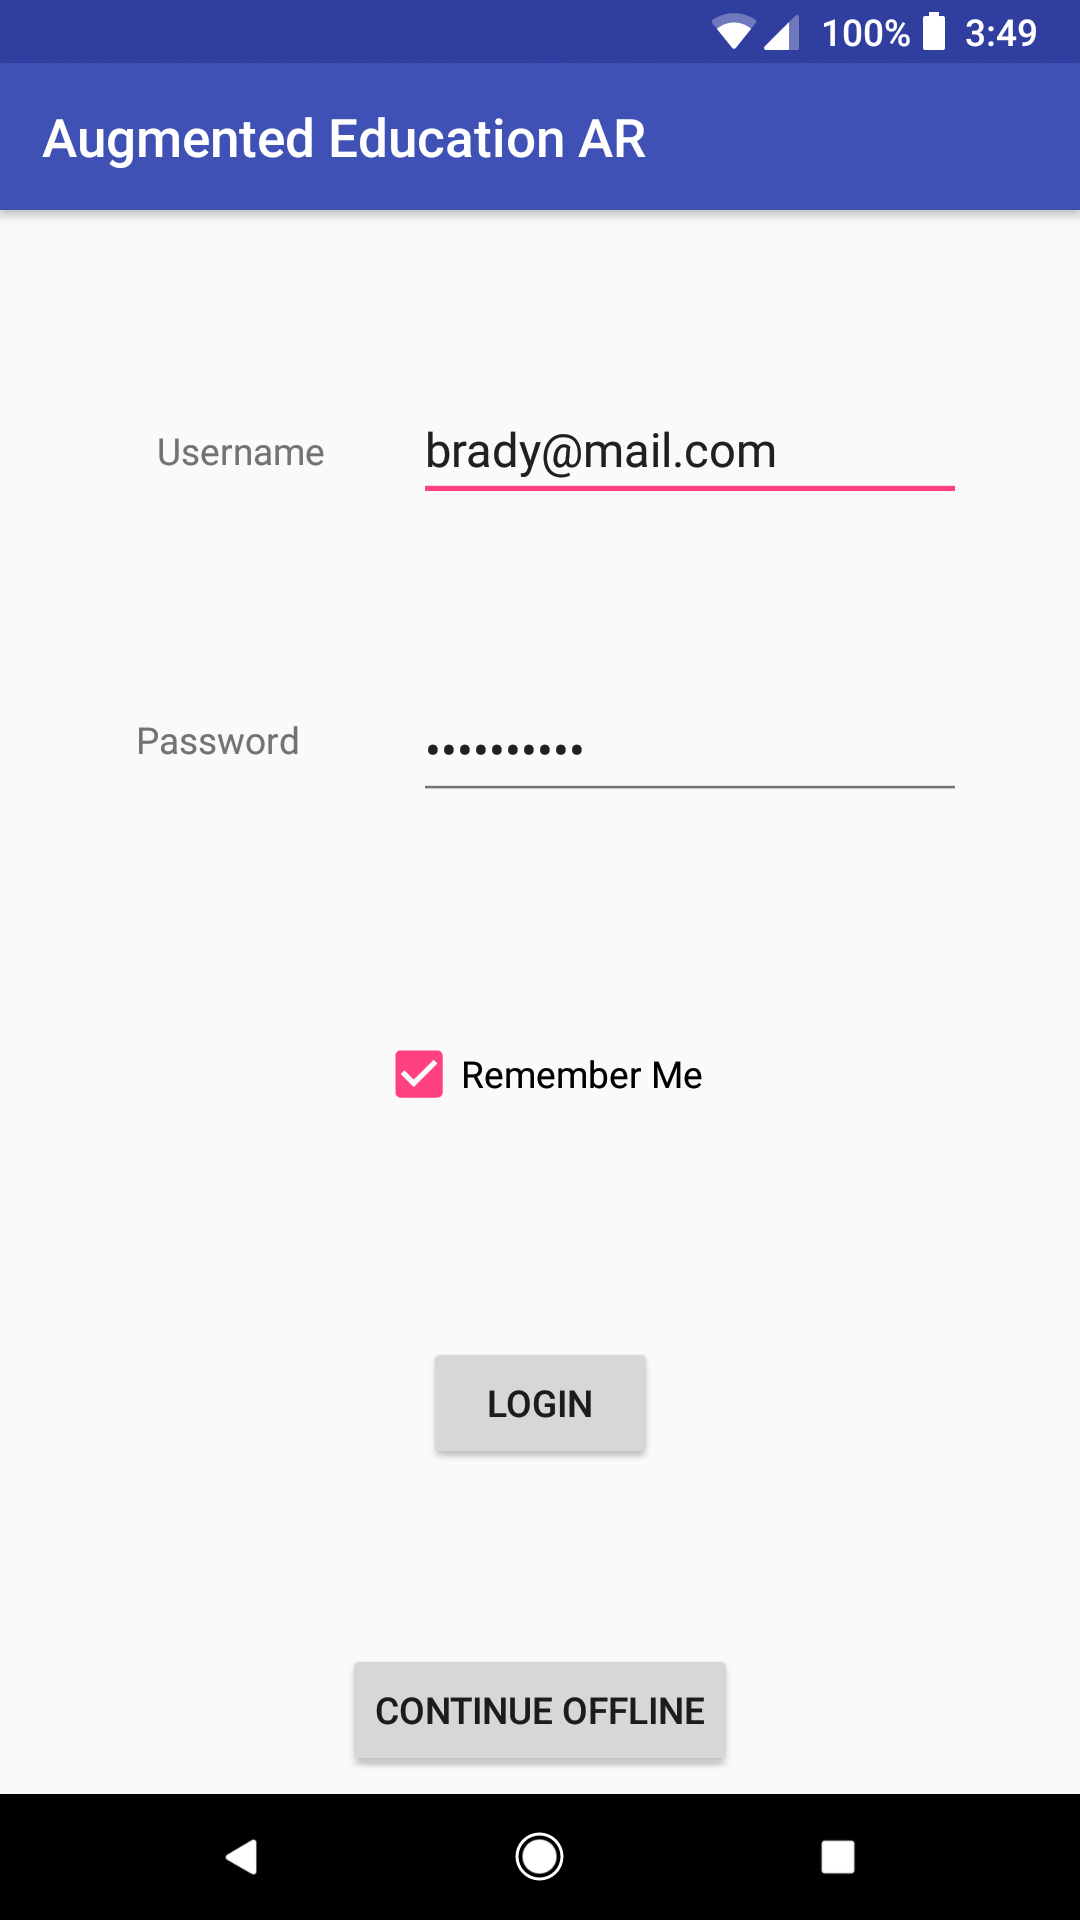
\includegraphics[width=0.5\textwidth]{Mobile/Mobile_MainActivity}
            \centering
            \caption{Mobile App - Login}
            \label{fig:mobileLoginActivity}
        \end{figure}

        \begin{figure}[H]
            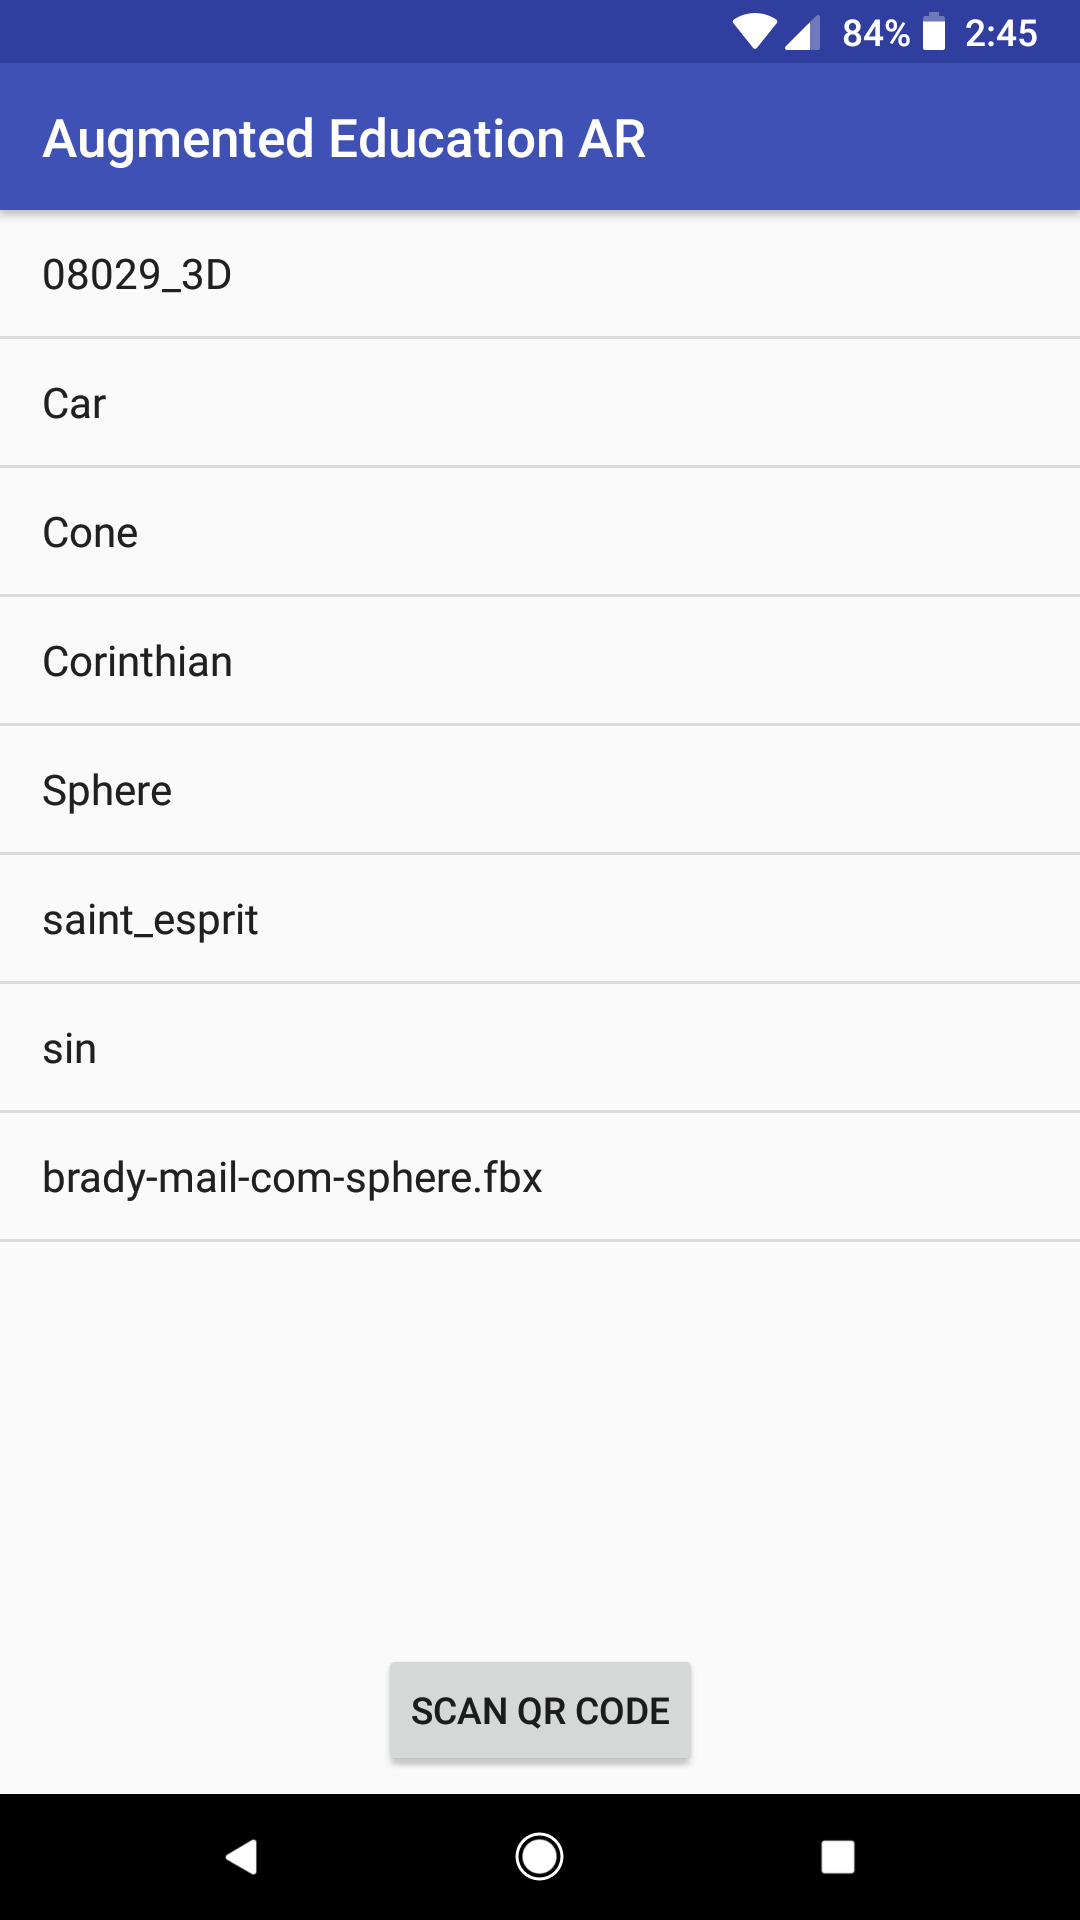
\includegraphics[width=0.5\textwidth]{Mobile/Mobile_ModelList}
            \centering
            \caption{Mobile App - Model Listing}
            \label{fig:mobileModelList}
        \end{figure}

        \begin{figure}[H]
            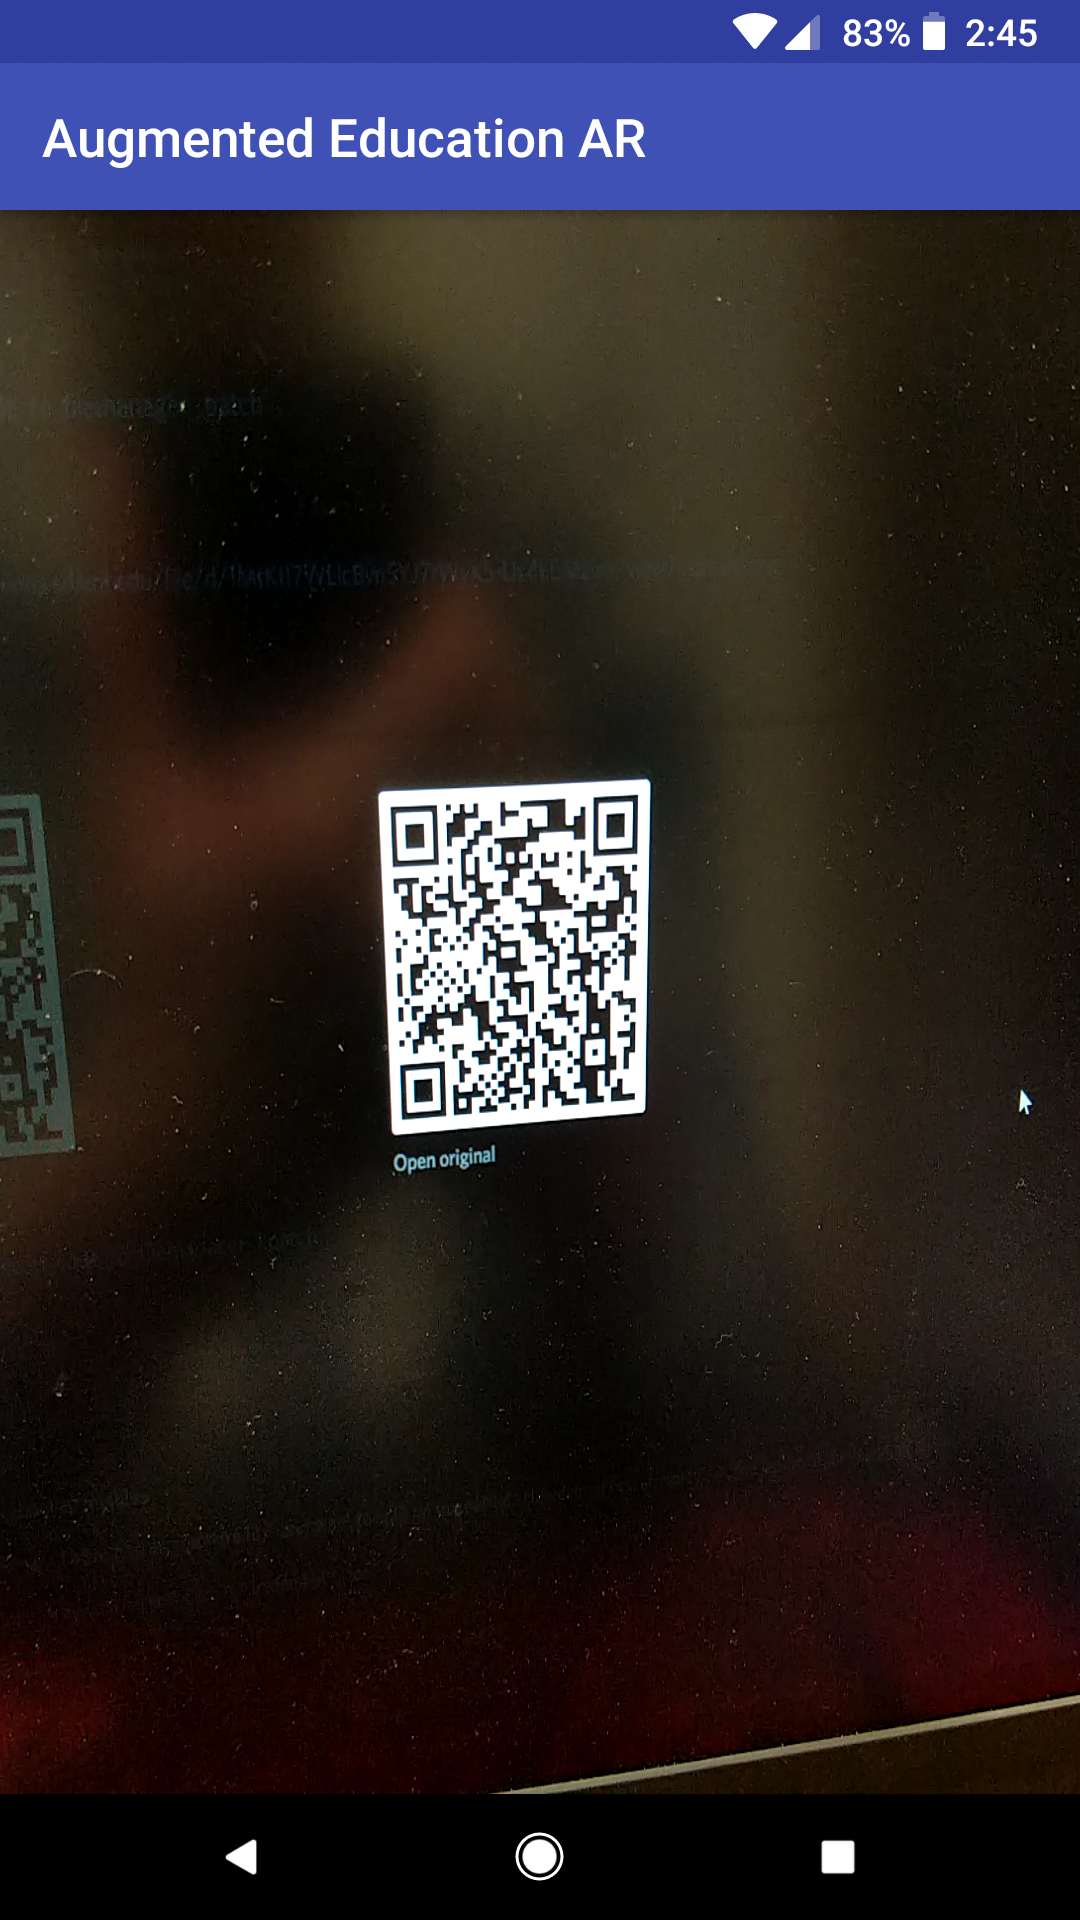
\includegraphics[width=0.5\textwidth]{Mobile/Mobile_QRScanning}
            \centering
            \caption{Mobile App - QR Code Reader}
            \label{fig:mobileQRScanning}
        \end{figure}

        \begin{figure}[H]
            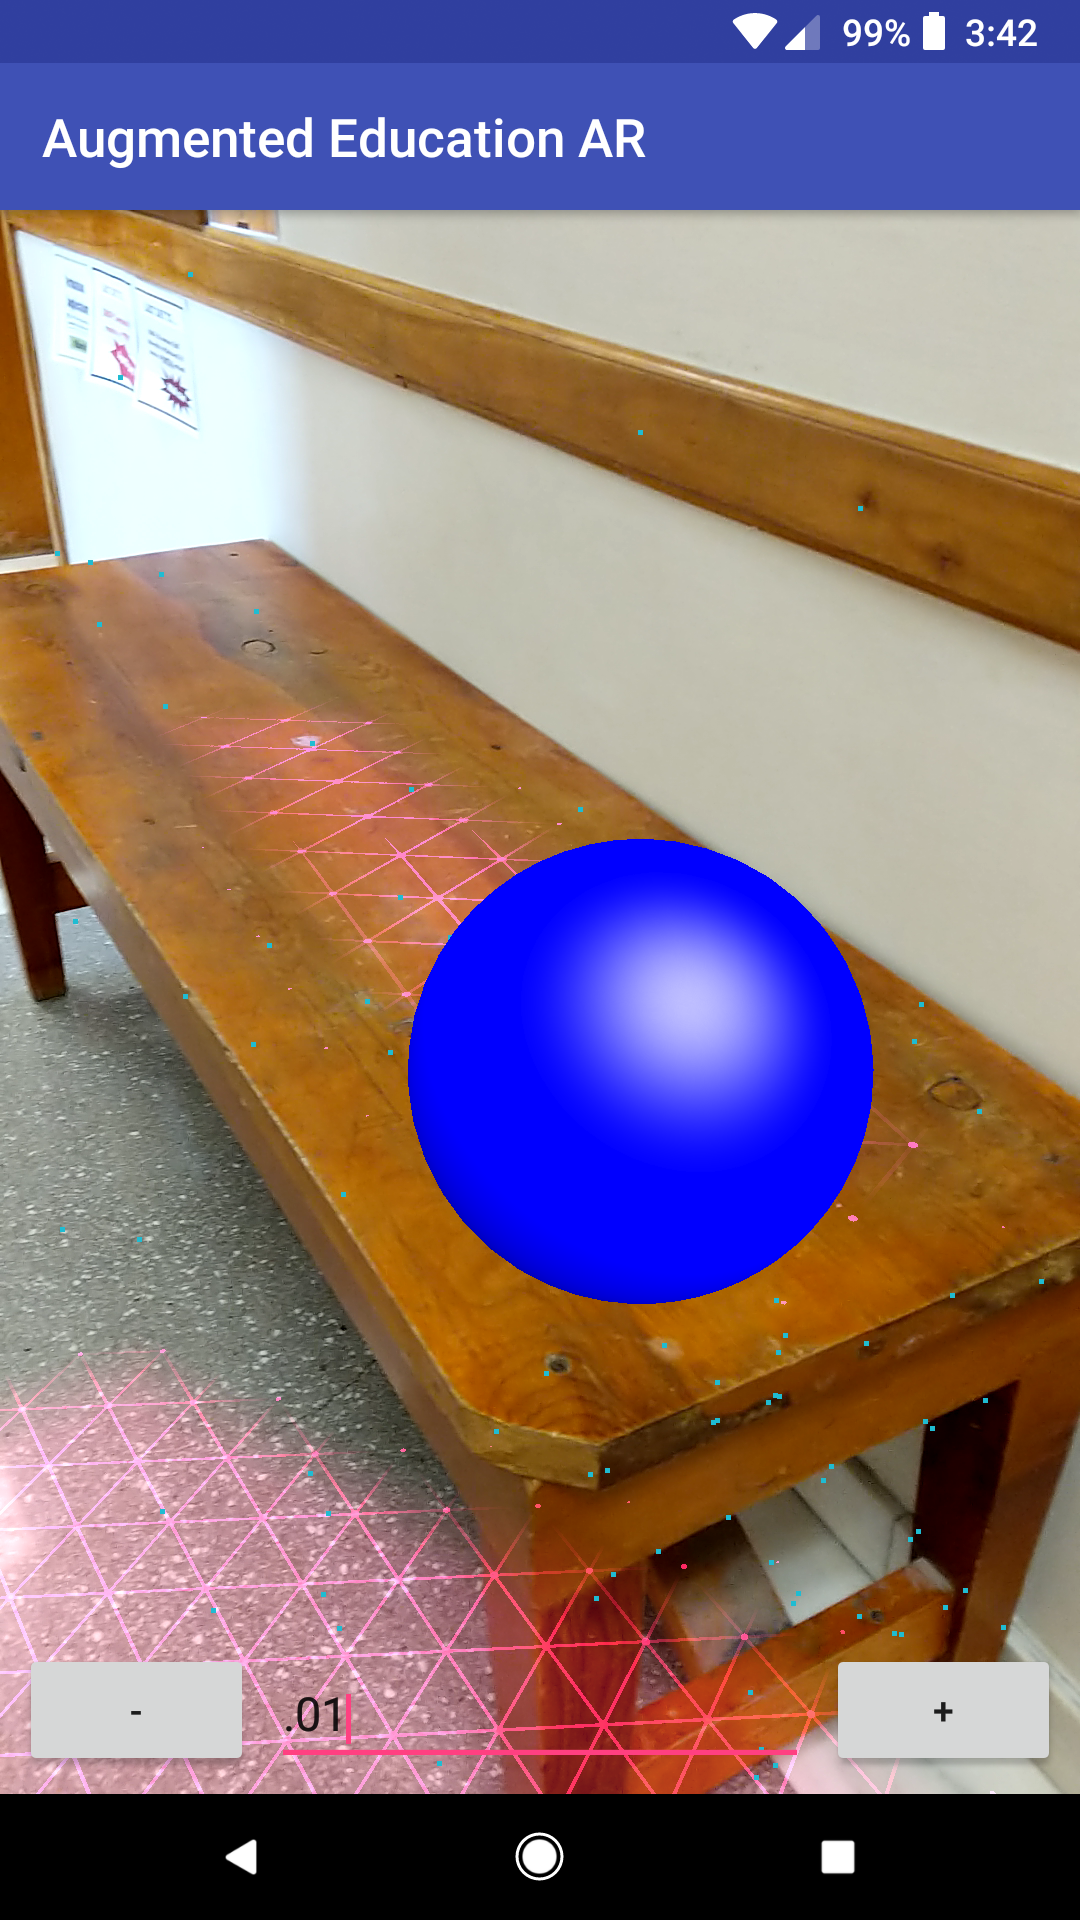
\includegraphics[width=0.5\textwidth]{Mobile/Mobile_BlueSphere}
            \centering
            \caption{Mobile App - AR Viewer}
            \label{fig:mobileModelViewer}
        \end{figure}

        \subsubsection{Code Structure}

